\subsubsection{UC5 - Configurazione alert}
\label{sssec:uc5}

\begin{figure}[h!]
  \begin{center}
    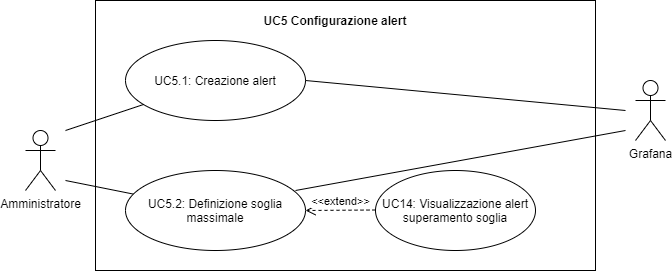
\includegraphics[width=10cm]{uc5.png}\\
    \caption{UC5 - Configurazione alert}%
    \label{fig:uc5}
  \end{center}
  \end{figure}

\begin{description}
	\item[Attore primario:] Utente amministratore.
	\item[Attore secondario:] Grafana.
	\item[Descrizione:] L'amministratore imposta degli alert con delle soglie di massima utilizzando i meccanismi offerti da Grafana.
	\item[Precondizione:]
	\begin{enumerate}
		\item L'amministratore ha configurato il plug-in correttamente(UC4);
		\item L'amministratore avvia il plug-in (UC4.1).
	\end {enumerate}
	\item[Scenario Principale:] L'amministratore definisce l'alert usando l'opzione "Crea alert"(UC5.1) che permette di definire una soglia per l'alert appena creato(UC5.2) tutto ciò usando i meccanismi offerti da Grafana.
	\item[Postcondizione:] L'amministratore ha impostato correttamente le soglie dei alert aggiunti tramite Grafana.
\end{description}

\paragraph{UC5.1 - Creazione alert}
\label{sssec:uc5.1}
\begin{description}
	\item[Attore primario:] Utente amministratore.
	\item[Attore secondario:] Grafana.
	\item[Precondizione:] L'amministratore si trova sul pannello di predizione.
	\item[Scenario Principale:] L'amministratore aggiunge un alert tramite l'opzione "Crea alert".
	\item[Postcondizione:] L'amministratore visualizza la pagina delle impostazione del pannello con la possibilità di aggiungere alert definiti da Grafana.
\end{description}

\paragraph{UC5.2 - Definizione soglia massimale}
\label{sssec:uc5.2}
\begin{description}
	\item[Attore primario:] Utente amministratore.
	\item[Attore secondario:] Grafana.
	\item[Precondizione:] L'amministratore ha selezionato l'opzione di inserimento di una soglia tramite l'opzione "Crea alert"(UC5.1).
	\item[Scenario Principale:] L'amministratore tramite Grafana definisce la soglia per l'alert e invia la conferma della creazione del suddetto.
	\item[Postcondizione:] L'amministratore ha impostato la soglia tale che parte l'alert impostato tramite Grafana.
	\item[Estensioni]: UC5.2 viene esteso nel caso d'uso UC14 con la visualizzazione di un messaggio di errore quando viene superata la soglia.
\end{description}
